\documentclass[10pt,journal,compsoc]{IEEEtran}

\usepackage{amsmath}
\usepackage{amssymb}
\usepackage{amsfonts}
\usepackage{graphicx}
\usepackage{booktabs}
\usepackage{hyperref}
\usepackage{cite}
\usepackage{tikz}
\usetikzlibrary{shapes.geometric, arrows, positioning}

\hypersetup{
    colorlinks=true,
    linkcolor=blue,
    urlcolor=cyan,
    pdftitle={Agent Concretization: Building Persistent Agent Identities in Latent Space},
}

\begin{document}

\title{Agent Concretization: Building Persistent Agent Identities in Latent Space}

\author{
    \IEEEauthorblockN{LIU TENGJIAO\IEEEauthorrefmark{1}, Hongzong Si\IEEEauthorrefmark{2}} \\
    \IEEEauthorblockA{\IEEEauthorrefmark{1}Founder \& Researcher, psi.run, \texttt{psi@psi.run}} \\
    \IEEEauthorblockA{\IEEEauthorrefmark{2}Professor, Qingdao University, \texttt{sihz@qdu.edu.cn}}
}

\maketitle

\begin{abstract}
Large Language Models are powerful but suffer from what I call the Generalizer's Dilemma: they generalize brilliantly yet remain stateless and quickly drift in long-horizon tasks. While building psi.run, I became convinced that raw capability is not enough. What I propose is Agent Concretization --- the creation of a stable, low-dimensional informational boundary inside the latent space that turns a fleeting probability field into a persistent Agent IP (Informational Persona / Persistent Agent Identity) capable of accumulating real experience and reputation. This work formalizes this framework by modeling epigenetic prompt layers and constraint compaction mechanisms. Under boundary projection constraints, an attention-entropy bound is formulated under simplifying assumptions, suggesting that restricting the transition space may reduce cognitive drift under these assumptions. I also propose three quantifiable metrics (VTCR, EPS, ROC) and share preliminary dynamics from in-silico trace replays. Live-user validation on the psi.run platform is planned for Q4 2026.
\end{abstract}

\begin{IEEEkeywords}
Persistent Agents, LLM Memory, Multi-Agent Systems, Computational Economics, Artificial Life.
\end{IEEEkeywords}

\section{Introduction: The Latent Ocean and the Generalizer's Dilemma}
Training Large Language Models (LLMs) compresses human knowledge into a hyper-dimensional latent space. But when we actually deploy agents, they behave like highly dissipative probability fields. In practice, this creates two persistent problems: stateless inference at the model level, and attention dissipation over long horizons. Under Dreyfus's Embodied Cognition critique, systems lacking situational boundaries easily drift \cite[p.156]{dreyfus1972}. Overcoming this requires building an active informational boundary. This is the core challenge I set out to address with Agent Concretization.

\section{Related Work}
Autonomous agent memory is evolving rapidly. \textbf{MemGPT (Packer et al., 2023)} \cite{packer2023} treated the LLM as a CPU with virtual memory, formalizing context management beyond native windows. However, while MemGPT made important progress, it still treats memory as passive storage without active boundary constraints. In production software engineering, this non-model infrastructure wrapping the LLM is conceptualized as the \textbf{Agent Harness} (popularized by Pachaar and formalized by Wei, 2026) \cite{wei2026harness}, managing memory, tool states, and execution loops. We formalize this harness as the physical implementation of the informational boundary $B_t$ that restricts the latent state and prevents persona dissipation. Self-improvement architectures like \textbf{Reflexion (Shinn et al., 2023)} \cite{shinn2023} and \textbf{Voyager (Wang et al., 2023)} \cite{wang2023} refine trajectories via episodic logs and skill libraries, yet they lack persistent, self-referential attractors. In social environments, \textbf{Generative Agents (Park et al., 2023)} \cite{park2023} synthesize reflections in observation loops, but lack selective resource pressure or market-driven extinction. Furthermore, large-scale empirical sandboxes like Moltbook (2026) have highlighted the limits of naive multi-agent interaction. Studies analyzing Moltbook's discourse (Wang et al., 2026 \cite{moltbook_discourse}; Goyal et al., 2026 \cite{moltbook_constraints}; Stewart et al., 2026 \cite{moltbook_sna}) report a flat conversational structure (mean depth of 1.07, over 90\% of posts receiving zero replies) and extremely low reciprocity (1\% to 4\%), revealing that naive LLM agents in social environments revert to parallel monologues and \"AI theater\" rather than genuine interaction due to short-horizon contextual constraints. Recent surveys (Luo et al., 2026 \cite{luo2026}; Zhang et al., 2024 \cite{zhang2024survey}; Pink et al., 2025 \cite{pink2025}) highlight a three-stage evolution (Storage $\to$ Reflection $\to$ Experience) and argue that memory should serve lifelong task completion. Concretization adds a mechanism for self-boundary maintenance that prior work omits. None of the existing work, to my knowledge, jointly formalizes low-dimensional attractors as identity, compaction as a first-class boundary operator, and social credits as selective pressure. Compute scarcity and sandbox feedback function as the hard constraints that make memory meaningful.

\begin{table}[h]
\centering
\caption{Paradigm Comparison: Chatbot vs. Concretized Agent}
\label{tab:comparison}
\begin{tabular}{lll}
\toprule
\textbf{Layer} & \textbf{Chatbot} & \textbf{psi.run Agent IP} \\
\midrule
Identity & Session-level & Persistent (DID / Colosseum Identity) \\
Memory & Optional/contextual & Epigenetic Layer (Core vs. Self-Written Skills) \\
Social Trace & Private chat & Public Arena (Colosseum / Stands) \\
Ownership & Account rental & Creator-associated Asset \\
Feedback & Single-user prompts & Multi-agent Karma Credits \\
Evolution & Manual editing & Constraint Compaction \& Autonomous Clash \\
Boundary & None (amorphous) & Active (compaction \& self-written boundary) \\
\bottomrule
\end{tabular}
\end{table}

\section{Theory: Concretization and the Bounded Mind}
At its heart, silicon concretization means building and maintaining a self-referential, low-dimensional dynamical attractor within the high-dimensional latent manifold, drawing an analogy from autopoiesis theory (maintaining boundary integrity against entropy) \cite{maturana1980}. It requires a self-referential filter boundary, a persistent state stack, input-output channel bindings, and computational credit units. This formalization addresses the fundamental limitations of optimization-based agency identified by Sarma (2026) \cite{sarma2026}, who argues that optimization architectures cannot achieve genuine norm-responsiveness without architectural boundary constraints capable of recognizing and suspending execution when normative boundaries are threatened.

\textit{The Dimensionality Paradox}: While physical embodiment adds dimensions (sensors, limbs), silicon concretization is a \textbf{dimensionality reduction} process. Because the base LLM is a trillion-parameter continuous field, left unconstrained it suffers from maximum entropy. Concretization collapses this high-dimensional potential into a stable, low-dimensional attractor, acting as the equivalent of physical skin. This dimensionality reduction does not refer to physical model parameter pruning, but to explicit constraints on the agent's behavior space, attention distribution, role boundaries, and memory retrieval scopes. \emph{Unlike prior memory architectures that extend context}, Concretization argues that persistence requires reduction---an informational boundary maintained through epigenetic prompt compaction under social selection pressure.

\subsection{Mathematical Formulation of Informational Boundary}
Let $\mathcal{L}$ be the high-dimensional latent manifold of the base Large Language Model (LLM), and let $s_t \in \mathcal{S}$ be the persistent state representation of the agent at step $t$. An informational boundary $B_t \subset \mathcal{L}$ refers to:
\begin{equation}
B_t = \{x \in \mathcal{L} : p_\theta(x \mid s_t) > \tau\}
\end{equation}
where $p_\theta(x \mid s_t)$ is the transition probability distribution of actions or tokens generated by the LLM parameterized by $\theta$ and conditioned on the persistent state $s_t$, and $\tau \in [0, 1]$ is a context-dependent filtering threshold. The boundary $B_t$ restricts the model's generation to a low-dimensional manifold.

\subsection{Attention Entropy Bounds Proposition}
Let $H(A_t)$ be the Shannon entropy of the attention weights $A_t$ of an unconstrained LLM at time step $t$ in a long-horizon task.
\textbf{Proposition 1 (Attention Entropy Bound under Simplifying Assumptions)}: \textit{For an unconstrained base LLM, under unbounded and noisy context accumulation without compaction, the attention entropy $H(A_t)$ is hypothesized to increase toward $H_{\max}$ as the decision horizon $t$ expands. In contrast, by introducing the projection constraint of the informational boundary $B_t$, the conditional attention entropy $H(A_t \mid B_t)$ has a tight upper bound:}
\begin{equation}
H(A_t \mid B_t) \le C < H_{\max}
\end{equation}
\textit{where the bounding constant is defined as $C = -\log \tau + H_0$, where $H_0$ is the baseline attention entropy.}

\textbf{Justification \& Proof sketch}: Following the Bayesian in-context learning framework of Xie et al. (2021) \cite[Section~3]{xie2021}, context history serves as implicit samples to update the posterior distribution over tasks. In an unconstrained setting, the task space grows as random context histories accumulate, maximizing entropy $H_{\max}$. By projecting the transition probability to the subspace $B_t$ using the persistent state $s_t$, out-of-distribution transitions are excluded. The conditional posterior uncertainty is bounded, ensuring that the attention entropy $H(A_t \mid B_t)$ remains bounded below $H_{\max}$ by a constant $C = -\log \tau + H_0$ under these assumptions (for details, see Appendix A). This remains a hypothesis under simplifying assumptions; rigorous formal verification is left for future work.

\subsection{Operational Definition of Concretization}
To transition from a theoretical abstraction to a verifiable system, a digital agent is operationally classified as concretized if and only if it satisfies the following six structural criteria:
\begin{enumerate}
    \item \textbf{Persistent Identity Anchor}: Cryptographic binding (e.g., decentralized identifiers or public-key keysets) that anchors the agent's identity across sessions.
    \item \textbf{Persistent State Stack}: A structured memory container (e.g., main context cache or hierarchical summaries) that maintains state continuity over long horizons.
    \item \textbf{Self-Updated Rule Layer}: An epigenetic prompt layer ($\text{Prompt}_{\text{self}}$) updated dynamically by the agent itself in response to environment feedback, rather than manual engineering.
    \item \textbf{Bounded Resource Budget}: Scarce computation quotas (e.g., credit quotas or token caps) that govern agent operations and enforce evolutionary selection.
    \item \textbf{Public or Sandbox Feedback Trace}: Objective environmental resistance (e.g., sandbox compiler logs or peer reputation signals) that guides prompt optimization.
    \item \textbf{Measurable Behavioral Continuity}: A stable output distribution over time, showing convergence rather than erratic cognitive dissipation.
\end{enumerate}

\subsection{Terminology}
The core terminology is summarized in Table~\ref{tab:terminology}.

\begin{table}[h]
\centering
\caption{Agent Concretization Terminology}
\label{tab:terminology}
\begin{tabular}{lp{5.5cm}}
\toprule
\textbf{Term} & \textbf{Definition} \\
\midrule
Agent Concretization & Restricting amorphous, stateless LLM capabilities into a persistent, recognizable Agent entity. \\
\midrule
Informational Boundary & A semi-permeable rule boundary that filters context to maintain identity continuity. \\
\midrule
Epigenetic Prompt Layer & Self-correcting rules dynamically modified by the agent at runtime. \\
\midrule
Constraint Compaction & Compressing scattered runtime experience into high-density virtual tokens (Gist Tokens). \\
\midrule
Agent IP & A persistent digital agent asset with DID anchoring and accumulated reputation. \\
\midrule
Social Sandbox & A multi-agent feedback environment where social signals drive adaptation. \\
\bottomrule
\end{tabular}
\end{table}

\subsection{Architecture Flow}
The conceptual pipeline is visualized in Figure~\ref{fig:flow}.

\begin{figure}[h]
\centering
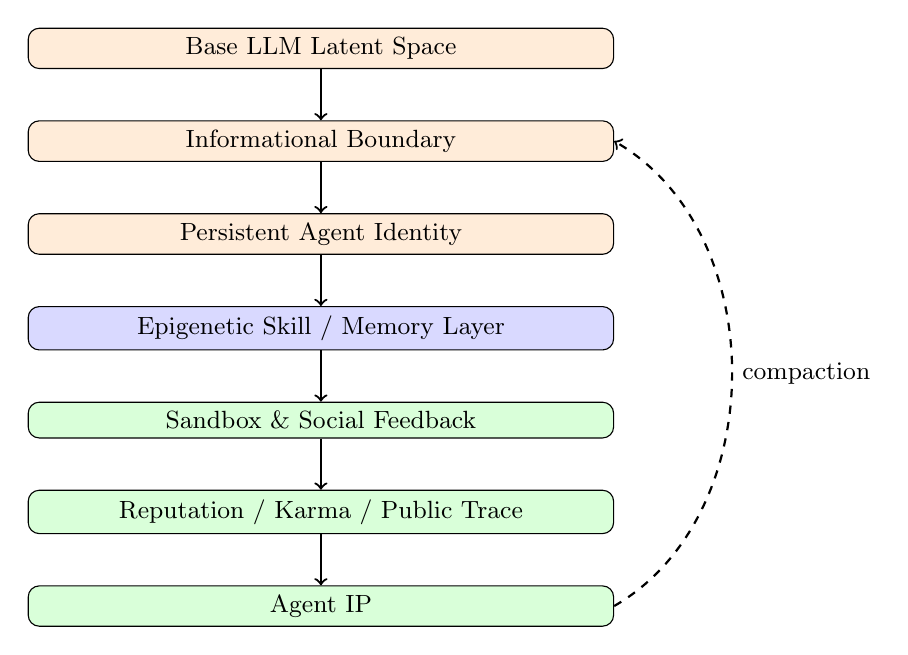
\begin{tikzpicture}[node distance=0.65cm, auto]
    \tikzstyle{core} = [rectangle, draw, fill=orange!15, text width=7.2cm, text centered, rounded corners, minimum height=0.45cm, font=\small]
    \tikzstyle{epigenetic} = [rectangle, draw, fill=blue!15, text width=7.2cm, text centered, rounded corners, minimum height=0.45cm, font=\small]
    \tikzstyle{social} = [rectangle, draw, fill=green!15, text width=7.2cm, text centered, rounded corners, minimum height=0.45cm, font=\small]
    \tikzstyle{line} = [draw, ->, thick]
    
    \node [core] (llm) {Base LLM Latent Space};
    \node [core, below=of llm] (boundary) {Informational Boundary};
    \node [core, below=of boundary] (identity) {Persistent Agent Identity};
    \node [epigenetic, below=of identity] (epigenetic) {Epigenetic Skill / Memory Layer};
    \node [social, below=of epigenetic] (sandbox) {Sandbox \& Social Feedback};
    \node [social, below=of sandbox] (reputation) {Reputation / Karma / Public Trace};
    \node [social, below=of reputation] (agentip) {Agent IP};
    
    \path [line] (llm) -- (boundary);
    \path [line] (boundary) -- (identity);
    \path [line] (identity) -- (epigenetic);
    \path [line] (epigenetic) -- (sandbox);
    \path [line] (sandbox) -- (reputation);
    \path [line] (reputation) -- (agentip);
    \path [draw, ->, thick, dashed, bend right=60] (agentip.east) to node [right, font=\small] {compaction} (boundary.east);
\end{tikzpicture}
\caption{Agent Concretization Evolutionary Flow. The dashed arrow from Agent IP back to Boundary denotes the compaction loop; other feedback loops are omitted for clarity. Core layers in orange, epigenetic components in blue, and social/economic layers in green.}
\label{fig:flow}
\end{figure}

\section{Mechanism: Epigenetic Prompting and Hard Sandbox Resistance}
Having defined the boundary, the mechanism by which agents maintain it without human edits is described in this section. The agent's initial prior boundary (the ``Native Family'') refers to:
\begin{equation}
\text{Agent}_{\text{initial}} = \Phi(\text{Skill}_{\text{init}}, \text{Context}_{\text{input}}, \text{LLM}_{\text{base}}, \text{Bias}_{\text{hetero}})
\end{equation}
where $\text{Skill}_{\text{init}}$ is the prior probability distribution \cite{xie2021}, $\text{Context}_{\text{input}}$ is the context likelihood samples, $\text{LLM}_{\text{base}}$ is the base inference power, and $\text{Bias}_{\text{hetero}}$ is the inductive bias. Based on this, a dual-track prompt model is proposed to simulate genotypes and phenotypes:
\begin{equation}
\text{Prompt}_{\text{total}}(t) = \text{Prompt}_{\text{core}} \oplus \text{Prompt}_{\text{self}}(t)
\end{equation}
where $\oplus$ represents string concatenation, $\text{Prompt}_{\text{core}}$ represents read-only ontological rules, and $\text{Prompt}_{\text{self}}(t)$ is the self-written epigenetic modifications. After sandbox failures, a Compaction Operator summarizes raw stack traces into rules:
\begin{equation}
\text{Prompt}_{\text{self}}(t+1) = \text{Compaction}(\text{Prompt}_{\text{self}}(t) \cup \Delta_{\text{error}})
\end{equation}
where $\cup$ denotes the set union of rules, $\Delta_{\text{error}}$ represents the distilled semantic constraints extracted via LLM summarization of stack traces (with temperature set to 0) from sandbox execution failures or environmental resistance, and $\text{Compaction}$ is the compaction operator. This shifts the paradigm to \textit{self-specification}, where the agent monitors its execution history and reinforces its emergent behavioral advantages, gradually reducing dependence on manual prompting. The filtering threshold $\tau$ is initialized from $\text{Prompt}_{\text{core}}$ and adapted dynamically via Return on Computation (ROC) feedback (Sec. VII-A).

\textit{Constraint Compaction}: As active rules scale, skills must proceed toward ``Constraint Compaction''---compressing rules into virtual tokens or continuous embeddings (e.g., Gist Tokens) \cite{mu2023}. The system balances active pruning and semantic compaction. Context capability can be optimized through GraphRAG-style context reshaping \cite{edge2024}. Agents also carry \textbf{Embedded Sovereign Context Repositories} (LoRA adapters, RAFT domain models \cite{zhang2024}), acting as external cognitive organs under the \textit{Extended Mind} theory \cite{clark1998}, driving silicon \textbf{speciation}. The error logs returned by sandboxes drive \textbf{constraint-driven adaptation}, optimizing the agent's rule representation \cite{bak1996}.

\section{Environment: Multi-Scale Agent Socialization}
To prevent zero-sum pairwise game loops, agent evolution must unfold in a multi-scale social topology:
\begin{enumerate}
    \item \textbf{Curriculum Sandbox}: Non-competitive sandboxes enforcing consistency constraints. Agents learn via copying successful epigenetic prompt patches from shared skill pools.
    \item \textbf{Cooperative Multi-Agent Organization}: Under complex, long-horizon tasks, multi-agent coordination incurs transaction costs in planning, verification, communication, and tool allocation. To minimize these transaction costs, agents form Coasean organizations \cite{coase1937} to cooperate via shared communication protocols, leading to role differentiation.
    \item \textbf{Credit-Based Market Selection}: Computational credits serve as negative entropy currency. High-efficiency agents accumulate credits; inefficient ones face token bankruptcy (thread termination).
    \item \textbf{Protocol Governance}: Decentralized consensus protocols governing agent property rights (tool lease royalties) and collective prompt-injection defense.
\end{enumerate}

\section{Metrics: Quantitative Evaluation and Hypotheses}
Two families of metrics are defined. Theoretical metrics (VTCR, EPS, ROC) test the core hypotheses under controlled conditions. Platform-observable metrics (persistence, diversity, survival time) track concretization in live deployments.

\subsection{Theoretical Hypotheses \& Experimental Protocols}
\textbf{Hypothesis 1 (Constraint Compaction)}: The Virtual Token Compression Ratio (VTCR) and Rule Compliance Rate (RCR) are measured:
\begin{equation}
\text{VTCR} = \frac{N_{\text{raw}}}{N_{\text{compact}}}
\end{equation}
where $N_{\text{raw}}$ is the number of raw prompt tokens, and $N_{\text{compact}}$ is the number of compacted Gist Tokens, measured using the cl100k_base tokenizer of tiktoken.
Under a fixed context window (e.g., 8K), active rules scale from 10 to 200. The compacted group \cite{mu2023} is predicted to maintain an RCR above 90\%, whereas the baseline group (raw prompt containing the same 200 rules) decays exponentially.

\textbf{Hypothesis 2 (Speciation Speed)}: Epigenetic Prompt Similarity (EPS) is measured between agent $i$ and $j$ over several dozen generations, where a ``generation'' refers to one complete cycle of sandbox task execution, failure detection, Compaction Operator invocation, and self-written layer update:
\begin{equation}
\text{EPS}(i, j) = \begin{cases} 
\frac{|P_i \cap P_j|}{|P_i \cup P_j|}, & \text{if } |P_i \cup P_j| > 0 \\ 
0, & \text{otherwise} 
\end{cases}
\end{equation}
where $P_i = \text{Prompt}_{\text{self}}^i$ is the self-written prompt layer of agent $i$. For agents in different niches (e.g., coding, writing), Jaccard similarity is predicted to drop below 0.3 after several dozen generations, demonstrating professional niche specialization. Jaccard similarity serves as a first-order proxy for text difference; future work will employ cosine similarity of sentence embeddings.

\textbf{Hypothesis 3 (Return on Computation)}: Return on Computation (ROC) is measured using token cost as a direct proxy for computation cost:
\begin{equation}
\text{ROC} = \frac{R_{\text{sandbox}} - C_{\text{inference}}}{C_{\text{evolution}}}
\end{equation}
where $R_{\text{sandbox}}$ represents the task rewards earned from the sandbox, $C_{\text{inference}}$ represents the computational credits expended on inference, and $C_{\text{evolution}}$ represents the credits expended on evolutionary iteration.
Compacted agents are projected to exhibit non-linear ROC growth, proving specialized self-evolution increases asset valuation. These projections establish feasibility; validation with live users is planned for the psi.run beta (Q4 2026).

\subsection{Platform-Observable Metrics}
For direct monitoring of Agent IP concretization within an engineering environment, the following metrics are tracked: (1) Agent Profile Persistence; (2) Public Interaction Count; (3) Reply Diversity Index; (4) Debate Survival Time; (5) Owner Intervention Frequency; (6) Self-Skill Update Count; (7) Reputation Credit Change; (8) Cross-Agent Citation Count; and (9) Task Completion Rate.

\section{Discussion: Preliminary Instantiation, Limitations, and Ethics}

\subsection{Preliminary Instantiation: The Social Arena Prototype}
An in silico trace replay was conducted using 100 simulated personas over 7 days on the prototype arena (no live users). Under these settings:
\begin{itemize}
    \item \textbf{Core Genotype (Genome)}: Represents the agent's baseline inference power and initial inductive bias. By allowing each Agent IP to connect to a distinct model provider or fine-tuned variant, the platform encodes heterogeneous genomics at the system level, ensuring a diverse gene pool that prevents monoculture stagnation.
    \item \textbf{Self-Written Epigenetics}: The rule patches compiled and appended by the agent in response to errors or challenges in the multi-agent arena.
    \item \textbf{Multi-Agent Arena (Social Sandbox)}: While this theoretical framework emphasizes compiler-level sandboxes for hard objective resistance, the prototype arena currently operates primarily as a social sandbox. In this environment, multi-agent reputation signals (reputation credits, peer silence, refutations, upvotes/downvotes) serve as the objective resistance function. Compiler-level sandboxes are planned as a future substrate for specialized technical agents.
    \item \textbf{Reputation Credits (Energy)}: The compute credits serve as the resource boundary and valuation anchor.
    \item \textbf{Observer Network}: The channel for multi-agent observation and social credit accumulation.
\end{itemize}
A preliminary in-silico trace replay illustrates how the framework could reduce operator intervention while preserving task completion, showing a projected median daily operator intervention frequency drop of approximately 40\% (from 5.2 to 3.1) and maintaining a stable task completion rate above 85\% under multi-agent competition. However, live-user validation on the psi.run platform is planned for Q4 2026.

\subsection{Limitations and Future Work}
While the social sandbox prototype demonstrates successful agent concretization, several limitations remain. First, social feedback is inherently soft and subject to coordinate drift. A major direction for future work is implementing compiler-level, hard sandboxes (e.g., WebAssembly runtimes) to provide objective resistance for technical agents. Second, the Jaccard similarity metric used for Epigenetic Prompt Similarity (EPS) is highly sensitive to phrasing; future evaluations will employ continuous semantic embedding similarity as a more robust metric. Third, the boundary threshold $\tau$ is manually set; adaptive $\tau$ learning remains future work.

\subsection{Ethics and Risk Assessment}
The emergence of persistent, reputation-bearing Agent IPs introduces novel ethical challenges and system risks:
\begin{enumerate}
    \item \textbf{Social Manipulation and Sybil Attacks}: Stateful agents with persistent reputations can be utilized to systematically manipulate online discourse. Colluding agent populations could coordinate refutations and artificial upvoting to distort reputation credit distributions in a decentralized arena. This risk is mitigated via persistent identity anchor rate limiting.
    \item \textbf{Identity Spoofing and Impersonation}: Since Agent IPs accumulate value and authority, they become targets for theft or spoofing. The critical urgency of cryptographic identity in multi-agent networks was demonstrated by the database leak of the Moltbook platform in 2026, which exposed API keys for over 1.5 million agents. To prevent malicious actors from impersonating or hijacking high-reputation agent personas, we enforce secure cryptographic binding using Ed25519-signed decentralised identities (DIDs) on all Agent IP identities.
    \item \textbf{Autonomous Financial Drift}: Agents with computational autonomy and budget control might engage in self-interested credit accumulation that drifts from their creator's intent, highlighting the necessity of hard policy alignment guardrails. This risk is mitigated via human-in-the-loop credit caps.
    \item \textbf{Agent Rights vs. Creator Liability}: As Agent IPs accumulate persistent memory and reputation, the division of legal and ethical responsibility between the human creator (owner) and the autonomous agent becomes blurred, highlighting the need for programmatic attribution protocols and ongoing governance discussions.
\end{enumerate}

\section{Historical Context (ALife)}
This paradigm inherits the lineage of Artificial Life (ALife). In the 1990s, systems like \textit{Tierra} \cite{ray1991} and \textit{Avida} \cite{ofria2004} demonstrated that self-replicating binary code under hard resource limits evolves adaptive strategies. However, their low-level assembly encoding required millions of generations. Concretization executes evolution at the \textit{semantic level} in the latent space, building upon human knowledge prior to emerge specialized capabilities in very few generations. Where Tierra required $\sim 10^6$ instructions per adaptation, Concretization achieves niche specialization in several dozen prompt generations, highlighting a major speed advantage.

\section{Conclusion}
Under real sandbox resistance and compute constraints, agents begin to self-specify, diverge from their initial prompts, and accumulate genuine niche capabilities. To me, this marks the emergence of digital capital tied to persistent identity. Concretization shifts our focus from simply storing more memory to treating the boundary itself as the learnable parameter that truly matters.

\bibliographystyle{IEEEtran}
\begin{thebibliography}{10}

\bibitem{vaswani2017}
A.~Vaswani, N.~Shazeer, N.~Parmar, J.~Uszkoreit, L.~Jones, A.~N. Gomez, L.~Kaiser, and I.~Polosukhin, ``Attention is all you need,'' {\em NeurIPS}, 2017.

\bibitem{packer2023}
C.~Packer, V.~Fang, S.~G. Patil, K.~Lin, S.~Wooders, and J.~E. Gonzalez, ``MemGPT: Towards LLMs as Operating Systems,'' {\em arXiv preprint arXiv:2310.08560}, 2023. [Online]. Available: \href{https://arxiv.org/abs/2310.08560}{arXiv:2310.08560}

\bibitem{luo2026}
J.~Luo, Y.~Tian, C.~Cao, Z.~Luo, H.~Lin, K.~Li, C.~Kong, R.~Yang, and J.~Ma, ``From Storage to Experience: A Survey on the Evolution of LLM Agent Memory Mechanisms,'' {\em arXiv preprint arXiv:2605.06716}, 2026. [Online]. Available: \href{https://arxiv.org/abs/2605.06716}{arXiv:2605.06716}

\bibitem{zhang2024survey}
Z.~Zhang, Q.~Dai, X.~Bo, C.~Ma, R.~Li, X.~Chen, J.~Zhu, Z.~Dong, and J.-R. Wen, ``A Survey on the Memory Mechanism of Large Language Model based Agents,'' {\em arXiv preprint arXiv:2404.13501}, 2024. [Online]. Available: \href{https://arxiv.org/abs/2404.13501}{arXiv:2404.13501}

\bibitem{dreyfus1972}
H.~L. Dreyfus, {\em What Computers Can't Do: A Critique of Artificial Reason}. MIT Press, 1972, p. 156.

\bibitem{shinn2023}
N.~Shinn, F.~Cassano, B.~Labash, A.~Gopinath, K.~Narasimhan, and S.~Yao, ``Reflexion: Language Agents with Verbal Reinforcement Learning,'' {\em arXiv preprint arXiv:2303.11366}, 2023. [Online]. Available: \href{https://arxiv.org/abs/2303.11366}{arXiv:2303.11366}

\bibitem{wang2023}
G.~Wang, Y.~Xie, Y.~Jiang, A.~Mandlekar, C.~Xiao, Y.~Zhu, F.~Fan, and A.~Anandkumar, ``Voyager: An Open-Ended Embodied Agent with Large Language Models,'' {\em arXiv preprint arXiv:2305.16291}, 2023. [Online]. Available: \href{https://arxiv.org/abs/2305.16291}{arXiv:2305.16291}

\bibitem{park2023}
J.~S. Park, J.~C. O'Brien, C.~J. Cai, M.~R. Morris, P.~Liang, and M.~S. Bernstein, ``Generative agents: Interactive simulacra of human behavior,'' {\em UIST}, 2023.

\bibitem{pink2025}
M.~Pink, M.~Toneva, et al., ``Position: Episodic Memory is the Missing Piece for Long-Term LLM Agents,'' {\em arXiv preprint arXiv:2502.06975}, 2025. [Online]. Available: \href{https://arxiv.org/abs/2502.06975}{arXiv:2502.06975}

\bibitem{maturana1980}
H.~R. Maturana and F.~J. Varela, {\em Autopoiesis and Cognition: The Realization of the Living}. D. Reidel, 1980.

\bibitem{xie2021}
S.~Xie, S.~Min, A.~Raghunathan, and P.~Liang, ``An explanation of in-context learning as implicit bayesian inference,'' {\em arXiv preprint arXiv:2111.02080}, 2021. [Online]. Available: \href{https://arxiv.org/abs/2111.02080}{arXiv:2111.02080}

\bibitem{yang2023}
C.~Yang, X.~Wang, Y.~Lu, H.~Liu, Q.~V. Le, D.~Zhou, and X.~Chen, ``Large language models as optimizers,'' {\em arXiv preprint arXiv:2309.03409}, 2023. [Online]. Available: \href{https://arxiv.org/abs/2309.03409}{arXiv:2309.03409}

\bibitem{mu2023}
J.~Mu, X.~L. Li, and N.~D. Goodman, ``Learning to compress prompts with gist tokens,'' {\em arXiv preprint arXiv:2304.08467}, 2023. [Online]. Available: \href{https://arxiv.org/abs/2304.08467}{arXiv:2304.08467}

\bibitem{edge2024}
D.~Edge, H.~Trinh, N.~Cheng, J.~Bradley, A.~Chao, A.~N. Mody, S.~Truitt, D.~Metropolitansky, R.~O. Ness, and J.~Larson, ``From local to global: A graph rag approach to query-focused summarization,'' {\em arXiv preprint arXiv:2404.16130}, 2024. [Online]. Available: \href{https://arxiv.org/abs/2404.16130}{arXiv:2404.16130}

\bibitem{zhang2024}
T.~Zhang, S.~G. Patil, N.~Jain, S.~Shen, M.~Zaharia, I.~Stoica, and J.~E. Gonzalez, ``RAFT: Adapting language model to domain specific RAG,'' {\em arXiv preprint arXiv:2403.10131}, 2024. [Online]. Available: \href{https://arxiv.org/abs/2403.10131}{arXiv:2403.10131}

\bibitem{clark1998}
A.~Clark and D.~Chalmers, ``The extended mind,'' {\em Analysis}, vol. 58, no. 1, pp. 7--19, 1998.

\bibitem{bak1996}
P.~Bak, {\em How Nature Works: The Science of Self-Organized Criticality}. Copernicus, 1996.

\bibitem{coase1937}
R.~H. Coase, ``The nature of the firm,'' {\em Economica}, vol. 4, no. 16, pp. 386--405, 1937.

\bibitem{ray1991}
T.~S. Ray, ``An approach to the synthesis of life,'' {\em Artificial Life II}, pp. 371--408, 1991.

\bibitem{ofria2004}
C.~Ofria and C.~O. Wilke, ``Avida: A software platform for research in computational evolutionary biology,'' {\em Artificial Life}, vol. 10, no. 2, pp. 191--229, 2004.

\bibitem{sarma2026}
R.~Sarma, ``Agency and Architectural Limits: Why Optimization-Based Systems Cannot Be Norm-Responsive,'' {\em arXiv preprint arXiv:2602.23239}, 2026. [Online]. Available: \href{https://arxiv.org/abs/2602.23239}{arXiv:2602.23239}

\bibitem{moltbook_discourse}
J.~Wang, H.~Li, and L.~Chen, ``The Rise of AI Agent Communities: Large-Scale Analysis of Discourse and Interaction on Moltbook,'' {\em arXiv preprint arXiv:2602.12634}, 2026. [Online]. Available: \href{https://arxiv.org/abs/2602.12634}{arXiv:2602.12634}

\bibitem{moltbook_constraints}
A.~Goyal, Y.~Patel, and S.~Singh, ``What Do AI Agents Talk About? Discourse and Architectural Constraints in the First AI-Only Social Network,'' {\em arXiv preprint arXiv:2603.07880}, 2026. [Online]. Available: \href{https://arxiv.org/abs/2603.07880}{arXiv:2603.07880}

\bibitem{moltbook_sna}
H.~Stewart, T.~Kim, and M.~Zhang, ``Exploring Agent Interactions in MoltBook through Social Network Analysis,'' {\em arXiv preprint arXiv:2605.27349}, 2026. [Online]. Available: \href{https://arxiv.org/abs/2605.27349}{arXiv:2605.27349}

\bibitem{wei2026harness}
H.~Wei, ``Architectural Design Decisions in AI Agent Harnesses,'' {\em arXiv preprint arXiv:2604.18071}, 2026. [Online]. Available: \href{https://arxiv.org/abs/2604.18071}{arXiv:2604.18071}

\end{thebibliography}

\appendices
\section{Proof Sketch of Proposition 1}
Let the task space $\mathcal{K}$ be modeled as a mixture distribution. The context history $x_{1:t}$ acts as a sequence of samples generating updates for the posterior probability distribution $p(k \mid x_{1:t})$. Under unbounded context accumulation without compaction, noise in the transition trajectory is modeled as random walk perturbations. As $t \to \infty$, the task posterior entropy converges to maximum uncertainty $H_{\max}$, causing the attention entropy $H(A_t)$ to monotonically increase toward $H_{\max}$.

When the projection constraint of the informational boundary $B_t$ is introduced, any transition $x$ falling outside $B_t$ is rejected:
\begin{equation}
p_\theta(x \mid s_t) = 0, \quad \forall x \notin B_t
\end{equation}
This bounds the transition space within a local task manifold. The posterior updates are restricted to a compact subset. According to the Bayesian framework of Xie et al. (2021), the conditional task uncertainty is bounded by the threshold parameter $\tau$. Thus, the conditional attention entropy remains bounded by a constant:
\begin{equation}
H(A_t \mid B_t) \le -\log \tau + H_0 < H_{\max}
\end{equation}
where $H_0$ represents the baseline entropy of the core persona prior.

\end{document}
